\documentclass[aspectratio=169, 8pt,t]{beamer}
\graphicspath{{figures/}} % Setting the graphicspath

% Theme settings
\usetheme{Madrid}
\usecolortheme{default}
\setbeamertemplate{navigation symbols}{}   % removes navigation symbols such as 'next page'
\setbeamertemplate{footline}{}             % remove line with name, date, page nr.
\setbeamercolor*{frametitle}{bg=white}     % remove background from frametitle
\usepackage{caption}
% \captionsetup[figure]{labelformat=empty}% redefines the caption setup of the figures environment in the beamer class.
\setbeamersize{text margin left=20pt,text margin right=10pt}
\usefonttheme[onlymath]{serif} % makes beamer math look like article math
\usepackage{hyperref}

%======================= title page info =======================
\title{News from NNPDF and the path to PDFs at N$^3$LO}
\subtitle{Based on 2401.08749, 2401.10319, and 2402.18635 }
\date{Joint Northern UK Journal Club  \\[0.1cm] 23 April 2024}
\author{Roy Stegeman}
\institute{\small The University of Edinburgh}


%======================= page numbering =======================
\addtobeamertemplate{navigation symbols}{}{ \usebeamerfont{footline}
  \insertframenumber / \inserttotalframenumber \hspace*{2mm} \\ \vspace*{1mm}
}


%=================================== colors ====================================
\definecolor{RoyBlue}{RGB}{22, 46, 69}
\definecolor{RoyGrey}{RGB}{64, 88, 128}

\newcommand{\hlme}[1]{{\color{red}\bf #1}} % highlight me

\setbeamercolor{structure}{fg=RoyBlue} % itemize, enumerate, etc
\setbeamercolor{frametitle}{fg=RoyGrey}
\setbeamercolor{section in head/foot}{bg=RoyBlue}


%======================= add progress dots to headline =========================
\setbeamertemplate{headline}{%
    \begin{beamercolorbox}[ht=4mm,dp=4mm]{section in head/foot}
        \insertnavigation{\paperwidth}
    \end{beamercolorbox}%
}%
\makeatother


%======================= add section title page ================================
\AtBeginSection[]{
  \begin{frame}
  \vfill
  \centering
    \usebeamerfont{title}\insertsection\par%
  \vfill
  \end{frame}
}


%=================================== titlepage =================================
\titlegraphic{\vspace*{6mm}
  
\includegraphics[height=1.5cm]{logos/edi_logo.png} \hspace{10mm}
  % 
\includegraphics[height=0.8cm]{logos/nnpdf_logo_official.pdf} \hspace{10mm}
  
\includegraphics[height=1.5cm]{logos/higgs_logo.jpg}
}

\defbeamertemplate{title page}{noinstitute}[1][]
{
  \vbox{}
  \vfill
  \begingroup
    \centering
    \begin{beamercolorbox}[sep=8pt,center,#1]{title}
      \usebeamerfont{title}\inserttitle\par%
      \ifx\insertsubtitle\@empty%
      \else%
        \vskip0.25em%
        {\usebeamerfont{subtitle}\usebeamercolor[fg]{subtitle}\insertsubtitle\par}%
      \fi%
    \end{beamercolorbox}%
    \vskip2em\par
    \begin{beamercolorbox}[sep=0pt,center,#1]{author}
      \usebeamerfont{author}\insertauthor
    \end{beamercolorbox}
  \begin{beamercolorbox}[sep=0pt,center,#1]{author}
    \usebeamerfont{institute}\insertinstitute
  \end{beamercolorbox}
  \vspace*{8pt}
  \vspace*{16pt}
    \begin{beamercolorbox}[sep=0pt,center,#1]{date}
      \usebeamerfont{date}\insertdate
    \end{beamercolorbox}\vskip0.5em
    {\usebeamercolor[fg]{titlegraphic}\inserttitlegraphic\par}
  \endgroup
  \vfill
}

\makeatletter
\setbeamertemplate{title page}[noinstitute][colsep=-4bp,rounded=true,shadow=\beamer@themerounded@shadow]
\makeatother


\begin{document}
{
\setbeamertemplate{headline}{} % remove headline from titlepage
\begin{frame}
  \titlepage
\end{frame}
}

\setbeamertemplate{enumerate items}[default]

\pgfdeclarelayer{bg}    % declare background layer
\pgfsetlayers{bg,main}  % set the order of the layers (main is the standard layer)


% SLIDES =======================================================================
\newcommand{\nn}{\vspace*{1em}}

\section*{PDF determination in NNPDF}

\begin{frame}{Introduce NNPDF}
\end{frame}



\section*{Motivation}

\begin{frame}{Motivation}
  PDFs, along with $\alpha_s$, are often a dominant source of uncertainty for predictions of LHC cross-sections
  \begin{columns}
    \begin{column}{0.49\textwidth}
      \vspace*{1em}

      Requirements for the next generation of PDFs are threefold:
      \begin{itemize}
        \item To exploit the impressive progress in N3LO calculations we require PDFs of the same order
        \item Missing higher order uncertainties (MHOUs) for some observables are larger than the experimental uncertainty and can thus no longer be neglected
        \item The level of precision aimed for at the LHC no longer allows neglecting EW corrections
      \end{itemize}

      \vspace*{1em}
      Focus on QED, but first briefly mention N3LO and MHOU
    \end{column}

    \begin{column}{0.49\textwidth}
      \begin{figure}
        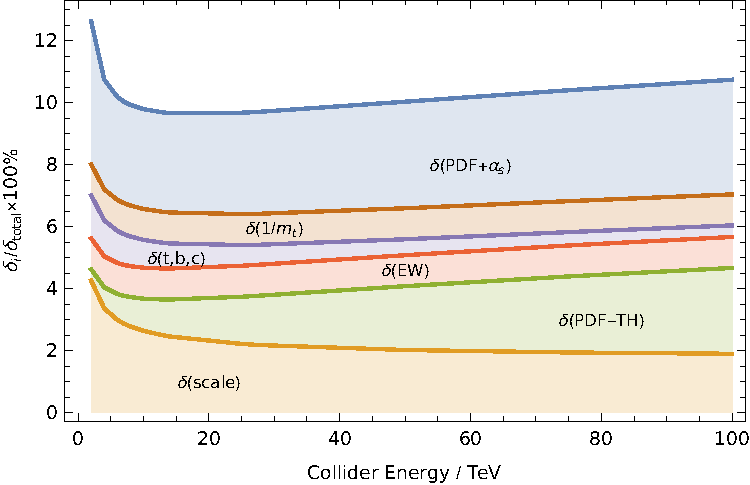
\includegraphics[width=0.8\textwidth]{figures/sources_of_unceratinty.pdf}
        \caption*{Uncertainties for inclusive Higgs production \\
        \color{gray}\small [HL-LHC: 1902.00134]}
      \end{figure}
    \end{column}
  \end{columns}
\end{frame}

\section{QED}

\section{MHOU}

\begin{frame}{Theory errors in a a PDF fit}
% include th covmat on same footing as exp covmat
% construct by varying fact and ren. scale var.
\end{frame}

\begin{frame}{Magnitude of theory uncertainties}
% show that for certain processes th unc is of same size as exp unc.
\end{frame}

\begin{frame}{Validate by comparing to known NNLO}
% show the validation plot
% we will see later the impact on the PDF/pheno
\end{frame}

\section{N$^3$LO}

\begin{frame}{Theory inputs for (approximate) N3LO}
% Needed:
% splitting functions
% VFNS matching conditions
% Matrix elements
  % DIS
  % Hadronic
% Not all available at N3LO, construct approximations where possible (and assess unc on the approximation)
\end{frame}


\begin{frame}{Splitting functions}
% construct approximate splitting functions satisfying known exact limits and results
% estimate incomplete missing higher order uncertainties (explain later how to include?)
% show splitting function plot that indicates convergence
  % point out IHOU are not negligible
\end{frame}


\begin{frame}{DGLAP evolution}
% show 1.65GeV to 100GeV evol plot (fig 2.8)
\end{frame}


\begin{frame}{DIS structure functions}
% Massless limit known up to N3LO
% massive can be parametrized joining the known limits
% show plot of C2 coefficients at NNLO (check) and aN3LO
\end{frame}


\begin{frame}{DIS variable flavor number scheme}
% PDF matching conditions almost completely known up to N3LO
\end{frame}


\begin{frame}{DIS variable flavor number scheme}
% nFONLL
% promote EKO + yadism
\end{frame}

\begin{frame}{Hadronic processes}
\end{frame}


\begin{frame}{Incomplete higher order uncertainties}
%
\end{frame}


\begin{frame}{NNPDF4.0 aN3LO}
% impact at PDF level of aN3LO and MHOU
\end{frame}

\begin{frame}{NNPDF4.0 aN3LO}
% impact at lumi level of aN3LO and MHOU
\end{frame}

\section{Phenomenology}

\begin{frame}{Higgs production}

\end{frame}


\begin{frame}{Drell-Yan}

\end{frame}


\begin{frame}{DIS at EIC}

\end{frame}


\section{Summary and outlook}
\begin{frame}{Incomplete higher order uncertainties}
  % outlook: combine N3LO+MHOU and QED
\end{frame}


\end{document}
